\chapter{Theory}
\section{Part 1: Determination of electrode distance d}

\subsection{Derivation of the effective dielectric permittivity}
\label{subsec.Derivationeffective}
The effective permittivity $\varepsilon_{\textrm{eff}}$ \nomenclature{$\varepsilon_{\textrm{eff}}$}{effective permittivity} is used to describe the permittivity of a composite material. This is necessary due to the fact that the assumption of homogeneity is not tenable for compound materials. The effective permittivity is defined as the ratio of the complex sample capacitance  $C^*$ 
\nomenclature{$C^*$}{complex capacitance [F]} to the vacuum capacitance $C_0$.\nomenclature{$C_0$}{vacuum capacitance [F]}

\begin{equation}
\varepsilon_{\textrm{eff}}(\omega) \equiv \frac{C^*(\omega)}{C_0} 
\end{equation}

Whereas the effective permittivity can be derived quite easily from the permittivities of the different materials for layered material geometries this is no more  possible for a complex setup. Thus, a numerical simulation is required as described in chapter \ref{sec.sim_vac_comsol}. In order to get $\varepsilon_{\textrm{eff}}$ the complex capacitance $C^*$ and the vacuum capacitance $C_0$ have to be obtained. While the former can be measured (voltage/current measurement) the latter has to be obtained with a numerical simulation. 
For the specimen in figure \ref{fig.specimen}, there are several geometric quantities that influence the vacuum capacitance. The most important factor is the distance of the electrodes as it may vary considerably (it is varied to obtain various levels of field stress in the material). As a consequence, a lookup table has to be created that allows an estimation of d if $C_0$ is given (for details on geometry see section \ref{sec.sim_vac_comsol}). 

 


\subsection{Interdependence between $\varepsilon$ and $\varepsilon_{\textrm{eff}}$} 
$\varepsilon$ is the permittivity of the dielectric. Both $\varepsilon$ and $\varepsilon_{\textrm{eff}}$ are complex parameters. Therefore, they can be written as $\varepsilon = |\varepsilon| e^{j \cdot \angle \varepsilon} $ and $\varepsilon_{\textrm{eff}} = |\varepsilon_{\textrm{eff}}| e^{j \cdot \angle \varepsilon_{\textrm{eff}}} $.	
The estimation of the dielectric permittivity of the epoxy in mixed epoxy-air configurations is usually based on the assumption that phase and magnitude of $\varepsilon$ and $\varepsilon_{\textrm{eff}}$ are decoupled. Thus, if one wants to estimate $\varepsilon$ of the dielectric material based on measurements of $\varepsilon_{eff}$ one has to investigate the interdependence of magnitude and phase of $\varepsilon$ and $\varepsilon_{\textrm{eff}}$ numerically. This effect can, in general, not be neglected as the simulation for a layered capacitors proves (see figure \ref{fig.layered}).  
\begin{figure}

	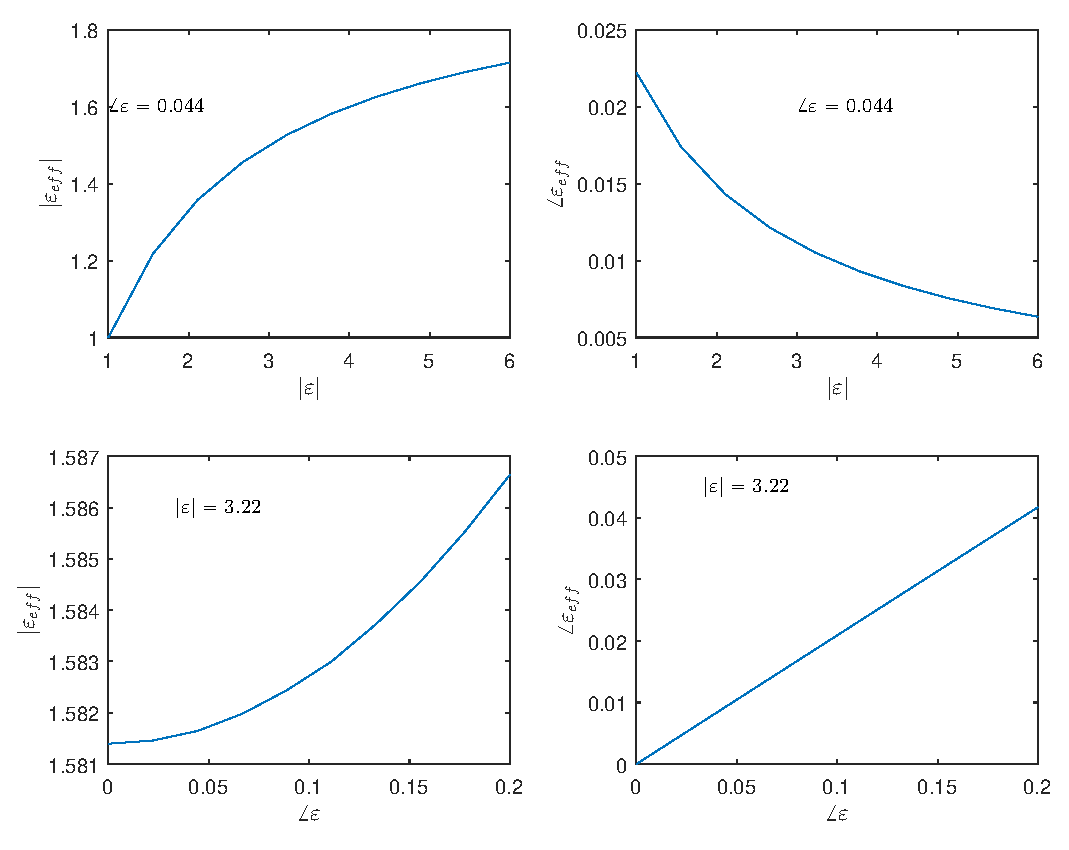
\includegraphics[width=0.8\textwidth]{figures/Theory/layereddielectrics.eps}
	\caption[Kurze Abbildungsbeschreibung]{Interdependeny of permittivity and effective permittivity in phase and magnitude for layered capacitor}
	\label{fig.layered}
\end{figure}
	
	
\section{Part 2: Suitability of current transformers for dielectric spectroscopy}
\subsection{Debye model}
The polarization effects in a dielectric material can be characterized by the complex relative permittivity. It is a frequency-dependent quantity. 
For linear materials the polarization can be described by a network model. The Debye-ansatz assumes that the rate of change $ \frac{dP}{dt}$ is proportional to the difference between the current polarization $P(t)$  and the polarization at infinity $P(\infty$). This results in an exponential relaxation of the polarization function that tends towards $P(\infty)$. In an alternating electric field this leads to a phase shift between the electric field $E(t)$ \nomenclature{$E$}{electric field strength [V/m]} and the  \nomenclature{$D$}{displacement field density}
electric displacement field $D(t)$.\newline
Formally, the lagging of the $\underline{D}$ field can be represented by using a complex proportionality factor between D and E. The underlined letter symbolizes the Fourier components.
\begin{equation}
 \underline{D}=\varepsilon \cdot \underline{E} = \varepsilon_{0}\varepsilon_{r}'\underline{E}-j\varepsilon_{0}\varepsilon_{r}''\underline{E}
\end{equation}


This exponential decay can be modeled with a \nomenclature{$P$}{polarization of material [$C/m^2$]} time constant of a resistor and a capacitor in series ($\tau=R_i \cdot C_i$). Therefore, an emulated dielectric comprises a vacuum capacitance, an additional capacitance $C_i$ and a resistor $R_i$ in series and a resistor $R_{\infty}$ for a stationary conduction current (DC conductivity). 


\subsubsection{Derivation of maximum tan($\delta$)}
The aim of this section is to derive the formula for the maximum tan($\delta$) of the Debye model in order to adjust its value to a desired one. The following formula was already stated in \ref{subsec.Derivationeffective}.
\begin{equation}
\varepsilon_{\textrm{eff}} (\omega) = \frac{C^*(\omega)}{C_0}
\end{equation}




\nomenclature{$\kappa$}{conductivity [S/m]}
For the delay of the dipole alignment given by the above \nomenclature{$\omega$}{angular frequency [rad/s]} mentioned debye-ansatz, one receives the following equations for the real and imaginary part of $\varepsilon$ \cite{Kuchler}. 
\begin{equation}
\varepsilon'_r = \varepsilon_{\infty} + \frac{\varepsilon_{\textrm{stat}}-\varepsilon_{\infty}}{1+(\omega \cdot \tau )^2}
\end{equation}


\begin{equation}
\varepsilon''_r = \omega \cdot \tau \cdot \frac{\varepsilon_{\textrm{stat}}-\varepsilon_{\infty}}{1+(\omega \cdot \tau )^2}
\end{equation}

The loss tangent \nomenclature{$\varepsilon_{stat}$}{static relative permittivity} is given by:
\begin{equation}
tan (\delta) = \frac{\kappa + \omega \cdot \varepsilon_0 \cdot \varepsilon _r ''}{\omega \cdot \varepsilon_0 \cdot \varepsilon _r '}
\end{equation}
It can be split up in one part for the polarization losses and another part for the conduction losses, which are given in the following equations. 
\begin{equation}
tan (\delta_{L}) = \frac{\kappa}{\omega \cdot \varepsilon_0 \cdot \varepsilon_r'} \newline
\end{equation}

\begin{equation}
tan (\delta_{pol}) = \frac {\varepsilon_r'' } {\varepsilon_r'}
\end{equation}


If measurements are carried out in the frequency domain from $10$ Hz to $10^{7}$ Hz, the complex dielectric function can be deduced from a measurement of the sample impedance $Z^*$ by using the following formula:

\begin{equation}
\varepsilon(\omega) = \frac{1}{j \omega  Z^*(\omega) C_0}
\end{equation}

The impedance of the chosen Debye model is given by 
\begin{equation}
Z_*(\omega)=[\frac{1}{R_\infty}+\frac{1}{R_i+\frac{1}{j \omega C_i}}+j \omega C_0]^{-1} = [\frac{1}{R_\infty}+\frac{j \omega C_i}{j\omega R_i  C_i+1}+j \omega C_0]^{-1}
\end{equation}
Hence,
\begin{equation}
\varepsilon^*(\omega)= \frac{[\frac{1}{R_\infty}+\frac{j \omega C_i}{j\omega C_i R_i  +1}+j \omega C_0]}{j \omega C_0} = \frac{1}{j \omega C_0 R_\infty}+ \frac{C_i/C_0}{j\omega C_i R_i  +1}+1
\end{equation}

The term for $\varepsilon$ is split up into a real and an imaginary part. 

\begin{equation}
\varepsilon_r' = 1+ \frac{C_i/C_0}{\omega^2 C_i^2 R_i^2 +1}
\end{equation}

\begin{equation}
\varepsilon_r'' = -j \left(\frac{1}{\omega C_0 R_\infty}+\frac{\omega C_i^2 R_i / C_0}{\omega^2 C_i^2 R_i^2 +1} \right)
\end{equation}

\begin{equation}
\tan(\delta) = tan(\delta_L) + tan( \delta_{Pol}) = \frac{\omega^2 \tau^2+1}{\omega C_0 R_\infty (2+ \omega^2 \tau^2)}+\frac{\omega \tau \Delta \varepsilon}{\varepsilon_{\textrm{stat}} + \omega^2 \tau^2}
\end{equation}

Its derivative is given by: 
\begin{align}
\begin{split}
\frac{\partial tan(\delta)}{ \partial \omega} & = \frac{[\omega C_0 R_\infty (2+\omega^2 \tau^2)]\cdot 2 \omega \tau^2 - (\omega^2 \tau^2 +1) [C_0 R_\infty (2+3 \omega^2 \tau^2)  }{[\omega C_0 R_\infty (2+\omega^2 \tau^2)]^2}\\
					      & + \frac{\tau \Delta \varepsilon [\varepsilon_{\textrm{stat}} + \omega^2 \tau^2] - 2 \omega \tau^2 [\omega \tau \Delta \varepsilon]}{[\varepsilon_{\textrm{stat}} +\omega^2 \tau^2]}
\label{eg:test}
\end{split}
\end{align}
					      
In order to find the maximum of tan($\delta_{pol}$) the first part of the term above, i.e. \eqref{eg:test}, is set equal to 0 to get an algebraic expression for the maximum value and its corresponding frequency. In the following, $\omega_{max}$ refers to the frequency at which $\tan(\delta_{pol})$ is maximum.

\begin{equation}
\tau \Delta \varepsilon [\varepsilon_{\textrm{stat}} + \omega^2 \tau^2] -2\omega \tau^2 [\omega \tau \Delta \varepsilon] = 0
\end{equation}
\begin{equation}
\omega^2 (\tau^3 \Delta \varepsilon -2 \tau^3 \Delta \varepsilon) = - \tau \Delta \varepsilon \cdot \varepsilon_{\textrm{stat}}
\end{equation}
\begin{equation}
\omega_{max}^2 = \frac{\tau \Delta \varepsilon \varepsilon_{\textrm{stat}}}{\tau^3 \Delta \varepsilon}
\end{equation}
\begin{equation}
\omega_{max} = \sqrt{\frac{\varepsilon_{\textrm{stat}}}{\tau^2}}
\end{equation}
\begin{equation}
\tan(\delta_{Pol})_{max} = \frac{\varepsilon_{\textrm{stat}} \Delta\varepsilon}{2\varepsilon_{\textrm{stat}}} = \frac{1}{2} \frac{\Delta \varepsilon}{\sqrt{\varepsilon_{\textrm{stat}}}}
\end{equation}
From here on, $\tan(\delta)$ refers to the pure polarization losses and it is assumed that the conduction losses can be neglected . This is usually the case for polar materials below a certain temperature. 

\section{Fourier Coefficients of trapezoidal pulse  train }

The Fourier coefficients of a trapezoidal pulse train are given by the following equation \cite{FaerberMVISS}. 
\begin{equation}
 U_n = \frac{2 U_0}{j \omega_n T} [e^{\frac{j \omega_n \tau}{2}} \textrm{sinc}{\frac { \omega_n \tau_r }{2}} -e^{\frac{-j \omega_n \tau}{2}} \textrm{sinc}{\frac{ \omega_n \tau_f}{2}}]
\end{equation}
$\tau$ stands for the FWHM (full width half maximum) of the trapezoidal pulses.
$\tau_r$ denotes the rise time  and $\tau_f$ is the fall time.

For the following analysis the following values are chosen:
\begin{equation}
\label{eg:taur}
 \tau_r = 0.5e^{-6 } s
  \end{equation}
  \begin{equation}
 \tau_f = 0.1e^{-6} s
  \end{equation}
 \begin{equation}
\tau= 1e^{-6} s
 \end{equation}
 \begin{equation}
 \label{eg:time}
  T=1e^{-3} s
 \end{equation}
 \newpage

The resulting frequency dependency can be seen in  \ref{fig.envelope}

\begin{figure}[H]
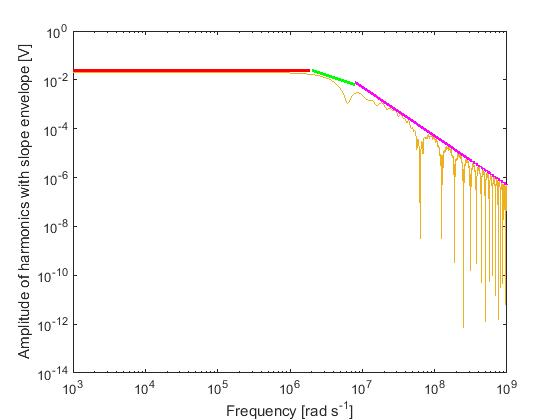
\includegraphics[width=\textwidth]{figures/Method/signal_simulation/envelope.jpg}
\caption[Kurze Abbildungsbeschreibung]{Fourier coefficients of the trapezoidal pulse train with respect to frequency. The solid lines represent the slopes of the envelopes that are caused by the individual 
cutoff frequencies of the parameters defined in \eqref{eg:taur} to \eqref{eg:time}}
\label{fig.envelope}
\end{figure}

Slopes of the curves: \newline
\begin{itemize}
 \item 0 on loglog plot for $\omega < \frac{2}{\tau}$\newline
\item -20dB/decade on loglog plot between $\omega = \frac{2}{\tau}$ and $\omega = \frac{2}{\tau_r}$ \newline
\item -40dB/decade on loglog plot after $\omega = \frac{2}{\tau_r}$\newline

\end{itemize}




	
\subsection{Devices for high frequency current measurement}
The most basic method for high frequency current measurement from DC up to the GHz region are shunt resistors. They make use of the the proportionality between the current and the voltage drop over the shunt. Besides, they are passive and have high bandwidths up to the GHz region. Another advantage is their ability to monitor DC currents. In order to keep the reduction of the current rate of rise in an acceptable range the self-inductance is often kept low by using coaxial shunts.\newline \cite{highdynamiccurrent}
A current transformer (CT) or pulse transformer is an instrument transformer that creates an AC-voltage on its secondary side that is proportional to the alternating current on its primary side. Most common are toroidal cores that are coiled. The secondary side has a low output resistance (usually 50 $\Omega$).
The principle setup of a current transformer is shown in figure \ref{fig.ct_setup}. 
\\CTs are as well suitable if the current on the primary side is too high to measure because the CT provides a voltage on the secondary side that is in a measurable range. A current transformer is suitable for current amplitudes from microamperes to megaamperes. A further advantage over a shunt resistance represents the galvanic isolation of the secondary side from the primary. This galvanic isolation prohibits large voltages on the secondary side (at measuring inputs) which might destroy the sensitive signal processing intrumentation connected to the circuit. \nomenclature{$\textrm{ADC}$}{Analog-to-Digital converter}
The transfer function for the current transformer can be calculated with the following differential equation, that is derived from Ampere's law (derivation based on: \cite{highdynamiccurrent}).\\
\begin{figure}
	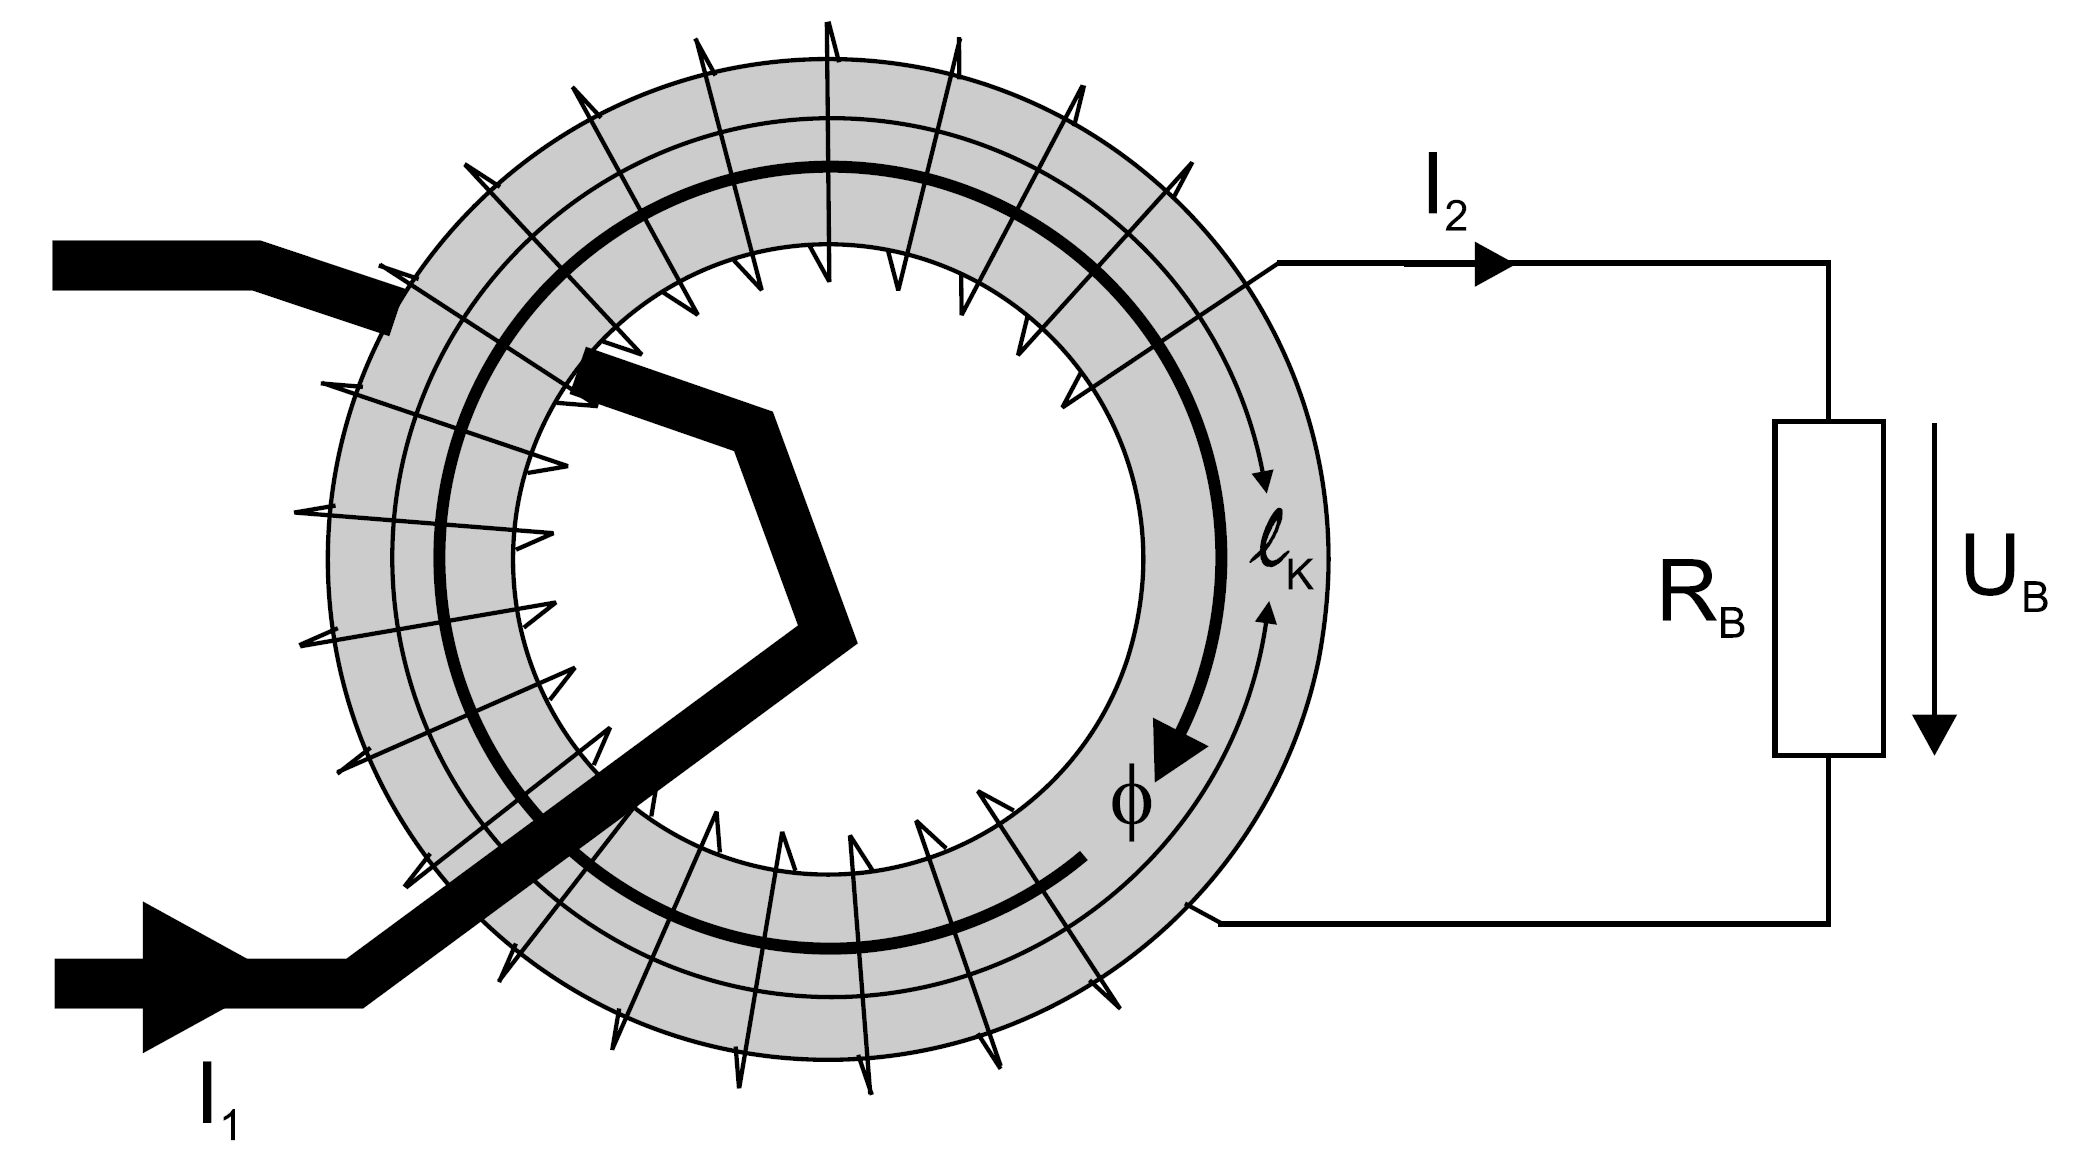
\includegraphics[width=0.8\textwidth]{figures/Theory/ct_setup}
	\caption[Kurze Abbildungsbeschreibung]{Structure of a current transformer with a primary current, a ring core and a secondary winding \protect\footnotemark}
	\label{fig.ct_setup}
\end{figure}
\footnotetext{figure taken from \cite{highdynamiccurrent}}

\begin{equation}
U_B(t) + \frac{L_2}{R_B} \cdot \frac{dU_B(t)}{dt}=\frac{N_1}{N_2} \cdot L_2 \cdot \frac{dI_1(t)}{dt}
\end{equation}
This results in a complex transfer function of: 
\begin{equation}
U_B(s) = R_B \cdot \frac{N_1}{N_2} \cdot \frac{s \frac{L_2}{R_B}}{s \frac{L_2}{R_B} +1} \cdot I_1(s)
\end{equation}

With the time constant $T=\frac{L_2}{R_B}$ this is a high-pass filter with a lower corner frequency of 
\begin{equation}
f_u= \frac{1}{2 \pi T} = \frac{R_B}{2 \pi L_2}
\end{equation}

For frequencies above the corner frequency the transfer function is:
\begin{equation}
G_CT(s) = \frac{U_B(s)}{I_1(s)}=R_B \cdot \frac{N_1}{N_2}
\end{equation}

This simplified model ignores the parasitic resistance and inductance of the primary and secondary side as well as stray capacitances between windings. 
For simplicity reasons the transfer function of a current transformer was assumed to be constant for the measurement, but this neglects the resistance and inductance of the primary and secondary side. 

\subsection{Noise Considerations}
\subsubsection{General}
The evaluation of noise added to the signal by the CT, the integrator (see section \ref{sec.integratormethod}, the BW-filter and the cables is of great importance as it limits the capability of resolving small values of tan($\delta$).
In order to quantify the desired signal compared to the background noise, the Signal-to-Noise Ratio (SNR) \nomenclature{$\textrm{SNR}$}{Signal-to-Noise-Ratio} can be measured. SNR is  the ratio of signal power over noise power. The power is proportional to the amplitude of the signal, hence \nomenclature{$\textrm{NF}$}{noise figure [dB]}
\begin{equation}
	\textrm{SNR}=\frac{P_{\textrm{signal}}}{P_{\textrm{noise}}} = \left[\frac{V_{\textrm{signal}}^{\textrm{rms}}}{V_{\textrm{noise}}^{\textrm{rms}}}\right]^2
\end{equation}
The degradation of the SNR is characterized by its input value over its output value, which is the Noise Figure (NF) and is indicated in dB.
\begin{equation}
	\textrm{NF} = 10\cdot \log\left(\frac{\textrm{SNR}_{\textrm{in}}}{\textrm{SNR}_{\textrm{out}}}\right)
\end{equation}
Thus, the amount of noise added by the components can be characterized by the NF. 


